\documentclass[spanish]{beamer}
\usepackage[spanish, activeacute]{babel}
\usepackage[latin1]{inputenc}
\usepackage{graphicx}

\usetheme{Ilmenau}

\title[Redes Neurales en Juegos]{Inteligencia Artificial II\\Redes Neurales en Juegos}
\author{Daniel Barreto \texttt{<daniel@ac.labf.usb.ve>}\\
        Kristoffer Pantic \texttt{<kristoffer.pantic@gmail.com>}}
\date{\today}

\begin{document}

\begin{frame}
\titlepage
\end{frame}

\begin{frame}[fragile]{Descripci�n General}
  \begin{itemize}
  \item Introducci�n
    \begin{itemize}
    \item Tipos de aprendizaje con redes neurales en juegos
    \end{itemize}

  \item Enfoques actuales
  
  \item Aplicaciones en estudio
    \begin{itemize}
    \item Aprendizaje en vivo (\emph{Online Learning})
    \item Aproximaciones centradas en el jugador
    \item Animaci�n inteligente de personajes
    \item Predicciones
    \item Estudios a nivel de inteligencia humana
    \end{itemize}
  \end{itemize}
\end{frame}

\begin{frame}{Introducci�n}
  \begin{figure}[htp]
    \centering
    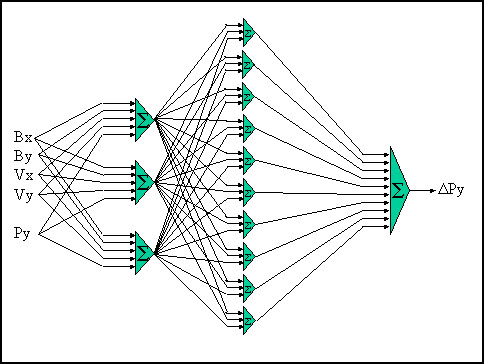
\includegraphics[scale=0.6]{media/neural.jpg}
  \end{figure}
\end{frame}

\begin{frame}{Tipos de aprendizaje en juegos}
  Particularmente para el aprendizaje artificial con redes neurales,
  podemos distinguir dos tipos aproximaciones:

  \begin{itemize}
  \item \emph{Offline learning.}
  \item \emph{Online learning.}
  \end{itemize}
\end{frame}

\begin{frame}{Tipos de aprendizaje en juegos}
  Otro tipo de categorizaci�n dada al aprendizaje artifical con redes
  neurales es:

  \begin{itemize}
  \item Aprendizaje supervisado
  \item Aprendizaje no supervisado
  \item Aprendizaje por reforzamiento
  \end{itemize}
\end{frame}

\begin{frame}{Enfoques actuales}
  
  \begin{itemize}
  \item Actualmente las redes neurales son poco usadas en juegos
    comerciales.
  \item En las versiones digitales de juegos de mesa como
    \emph{Othello}, \emph{Ajedrez}, \emph{Backgammon}, etc. es mas
    com�n el uso de redes neurales, por ser juegos de estrategia.
  \end{itemize}

  Los juegos de mesa suelen ser juegos m�s lentos con menos cambios de
  ambiente y mucha estrategia, mientras que en los juegos modernos hay
  muchos otros factores con que lidear aparte de la inteligencia
  artificial.
\end{frame}

\begin{frame}{Enfoques actuales}
  A pesar del poco uso, las redes neurales actualmente estan siendo
  utilizadas en el proceso de toma de decisiones de los agentes.
  \begin{figure}[htp]
    \centering
    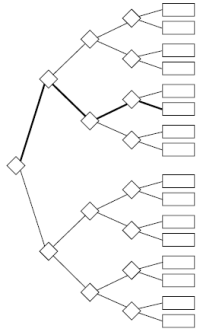
\includegraphics[scale=0.3,angle=270]{media/decision-tree.png}
  \end{figure}
  Los agentes procesan lo recibido por sus sensores, y a trav�s de una
  red entrenada (usualmente de forma \emph{offline}) toman acciones a
  partir de su output.\\

  Esto supone ahorro de c�digo y complejidad de maquinas de estados y
  agentes basados en reglas.
\end{frame}

\begin{frame}{Ejemplos de enfoques actuales}
  \begin{center}
    \textbf{Colin McRae Rally 2}
  \end{center}
  \begin{figure}[htp]
    \centering
    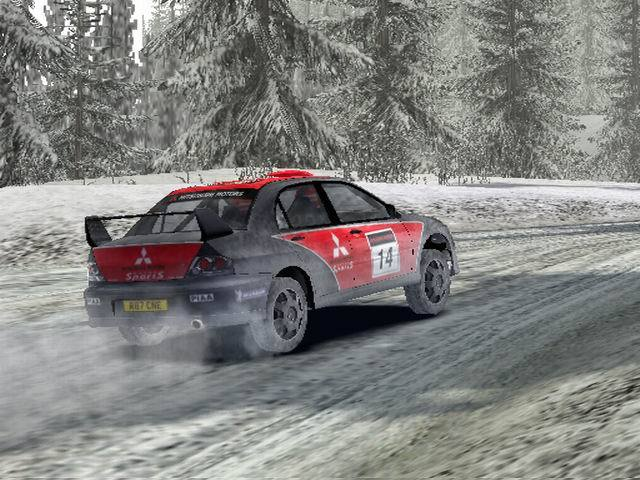
\includegraphics[scale=0.3]{media/colin-mcrae-rally.jpg}
  \end{figure}
\end{frame}

\begin{frame}{Ejemplos de enfoques actuales}
  \begin{center}
    \textbf{The Sims}
  \end{center}
  \begin{figure}[htp]
    \centering
    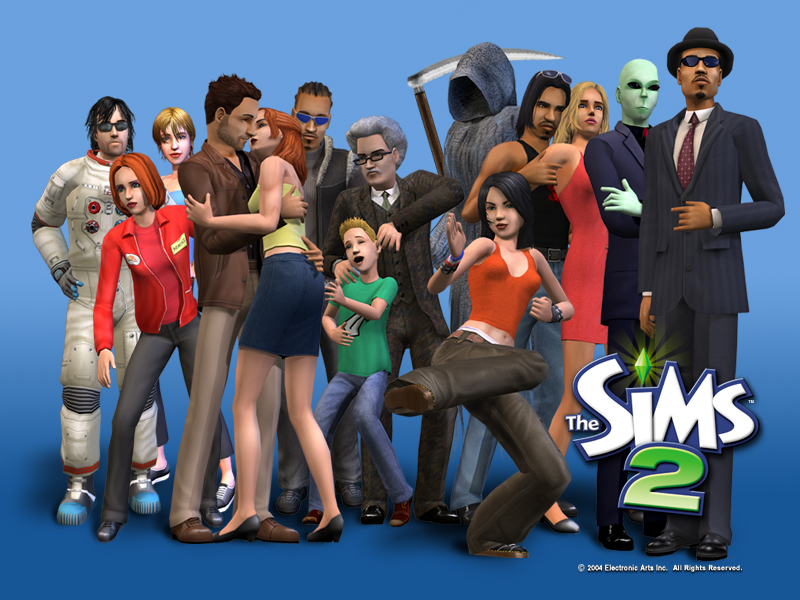
\includegraphics[scale=0.25]{media/the-sims.jpg}
  \end{figure}
\end{frame}

\begin{frame}{Ejemplos de enfoques actuales}
  \begin{center}
    \textbf{Quake III}
  \end{center}
  \begin{figure}[htp]
    \centering
    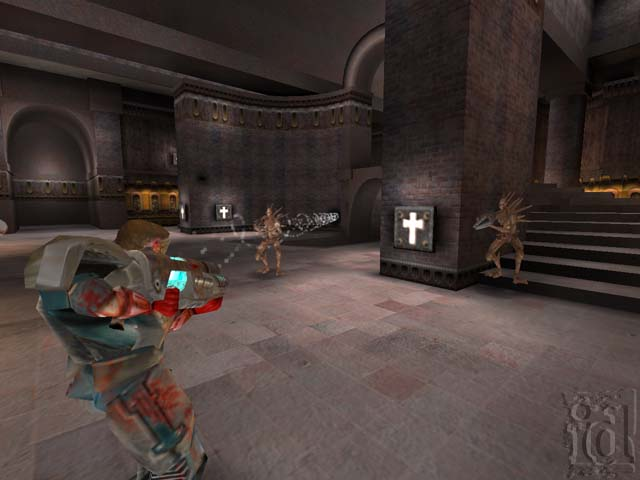
\includegraphics[scale=0.3]{media/quake3.jpg}
  \end{figure}
\end{frame}

\begin{frame}{Ejemplos de enfoques actuales}
  \begin{center}
    \textbf{Black and White}
  \end{center}
  \begin{figure}[htp]
    \centering
    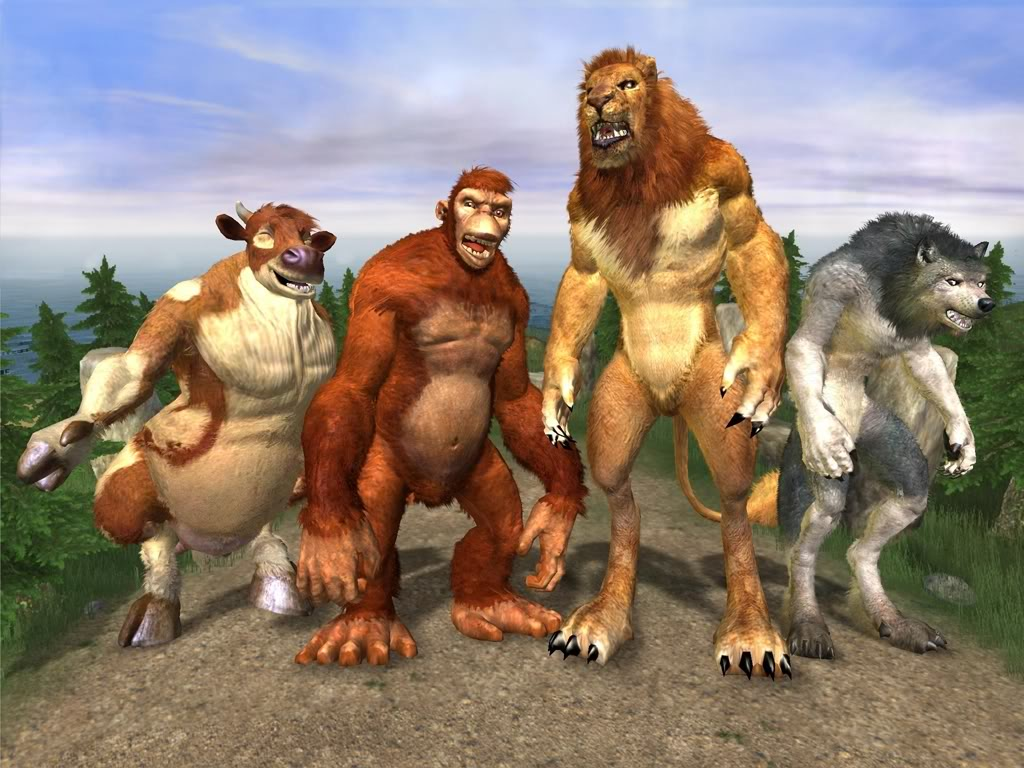
\includegraphics[scale=0.2]{media/black-and-white.jpg}
  \end{figure}
\end{frame}

\begin{frame}{Ejemplos de enfoques actuales}
  \begin{center}
    \textbf{Creatures}
  \end{center}
  \begin{figure}[htp]
    \centering
    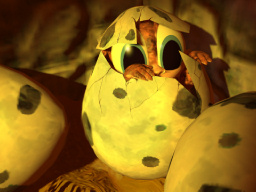
\includegraphics[scale=3.2]{media/creatures.jpg}
  \end{figure}
\end{frame}

\begin{frame}{Aplicaciones en estudio} 
  \begin{itemize}
  \item Aprendizaje en vivo (\emph{Online Learning})
  \item Aproximaciones centradas en el jugador
  \item Animaci�n inteligente de personajes
  \item Predicciones
  \item Estudios a nivel de inteligencia humana
  \end{itemize}
\end{frame}

\begin{frame}{Aprendizaje en vivo (\emph{Online Learning})}

  \emph{Online Learning:} Entrenar la red neural con los datos
  recibidos por el jugador, una vez que el juego ya ha sido totalmente
  desarrollado.

  \begin{itemize}
  \item \textbf{Ganancias de desarrollar �sta t�cnica}
    \begin{itemize}
    \item Adaptaci�n din�mica al comportamiento de los jugadores.
    \item Adaptaci�n din�mica al nivel de juego de los jugadores.
    \item Puede ser usado para contrarrestar los jugadores que
      obtienen puntos en el juego haciendo trampa.
    \end{itemize}
  \end{itemize}
\end{frame}

\begin{frame}{Aprendizaje en vivo (\emph{Online Learning})}
  \begin{itemize}
  \item \textbf{Obst�culos para desarrollarla}
    \begin{itemize}
    \item Resultados impredecibles.
    \item Introducci�n din�mica de bugs en el juego.
    \item El entrenamiento puede ser requerido muchas veces para poder
      adaptar la red neural y balancearla a los requerimientos del
      juego.
    \item El entrenamiento puede llegar a ser muy lento.
    \end{itemize}
  \end{itemize}
\end{frame}

\begin{frame}{Aproximaciones centradas en el jugador}
  \begin{itemize}
  \item Aproximaciones de aprendizaje sobre el jugador en si, para
    buscar mejorar la ``Experiencia de juego''.
  \item Se busca usar el poder que tienen las redes neurales para
    reconocer patrones y utilizarlos en las actuaciones de los
    jugadores.
  \item Se busca hacer que los juegos puedan tener un rango mas ancho
    de preferencias de los usuarios.
  \end{itemize}
\end{frame}

\begin{frame}{Aproximaciones centradas en el jugador}
  Algunas aproximaciones que se pueden tomar son las siguiente:

  \begin{itemize}
  \item Usar los tiempos de juego de un jugador, sus reacciones, sus
    decisiones tomadas, estilo de juego, precision de sus disparos,
    promedio de vida, etc. como parte de los inputs de una red neural
    que se entrena \emph{offline} para determinar ciertos modelos de
    jugadores, y en base a esto ajustar el entorno de juego.

  \item Aprovechar la capacidad de las redes neurales para realizar
    ``Algor�tmos de Clustering'' y agrupar a diferentes tipos de
    jugadores usando datos de su participacion dentro del juego,
    ajustandolos a ciertos perfiles de usuarios pre-establecidos.
  \end{itemize}
\end{frame}

\begin{frame}{Animaci�n inteligente de personajes}
  Actualmente las animaciones que pretenden simular a los humanos
  se limitan a ciertas expresiones faciales o movimientos corporales
  previamente grabadas usando actores humanos pero �sto acarrea
  grandes costos humanos y poca precisi�n debido a la tecnolog�a
  actual disponible para la captura de movimiento.
\newline
\newline
  El uso de redes neurales permite simular ciertos movimientos a
  partir de algunas capturas b�sicas.
\end{frame}
\begin{frame}{Animaci�n inteligente de personajes}
  Ventajas del uso de esta t�cnica:
  \begin{itemize}
    \item Ahorro de tiempo de trabajo para los animadores.
    \item Mayor versatilidad en las animaciones.
    \item Permite la creaci�n de animaciones en tiempo real, lo
      cual agrega realismo al juego.
  \end{itemize}
\end{frame}
\begin{frame}{Animaci�n inteligente de personajes}
  \begin{center}
    \textbf{Animaciones real�sticas de humanos}
  \end{center}
  \begin{figure}[htp]
    \centering
    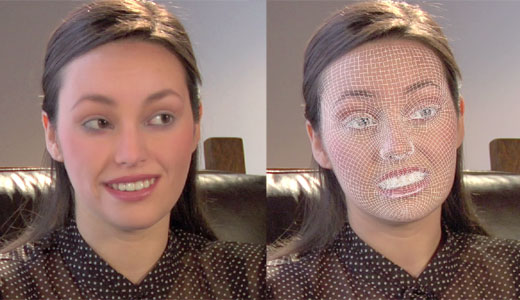
\includegraphics[scale=0.5]{media/image_metrics_emily.jpg}
  \end{figure}
\end{frame}

\begin{frame}{Predicciones}
  A partir de una red neural debidamente entrenada podemos simular
  la reacci�n de un cierto ambiente ante unos est�mulos y as� posiblemente
  predecir la acci�n resultante.
  \newline
  \newline
  Tienen varias aplicaciones en otras �reas:
  \begin{itemize}
    \item Finanzas.
    \item Predicci�n del clima.
    \item Comsumo de energ�a el�ctrica.
    \item Forecast de ventas.
    \end {itemize}
\end{frame}
\begin{frame}{Predicciones}
  En el �rea de juegos no son comunes pero pueden ser utilizados
  para: 
  \begin{itemize}
    \item En juegos de estrategia al decidir las acciones de un oponente
      computarizado prediciendo la pr�xima acci�n del jugador.
    \item En juegos de primera persona los "bots" pueden actuar en
      funci�n del movimiento del jugador para contrariarlo.
  \end{itemize}
  La predicci�n ofrece la ventaja de que permite tener una respuesta
  no-determin�stica a una situaci�n y por lo tanto permite la implementaci�n
  de oponentes computarizados m�s interesantes y variados.
\end{frame}

\begin{frame}{Estudios a nivel de inteligencia humana}
  Consisten en simular mediante el uso de inteligencia artificial
  las acciones y decisiones que podr�an ser tomadas por un humano.
  \newline
  \newline
  En los juegos se pueden usar las redes neurales para crear un jugador 
  virtual que permita el entrenamiento off-line de las dem�s redes del 
  sistema y que se pueda adaptar a cualquier juego donde sea configurado 
  lo cual permitir�a que dicho entrenamiento pueda formar parte del
  perfil de un jugador para una plataforma de juego.
\end{frame}

\end{document}